%===================================== CHAP 7 =================================
\chapter{Investigation of resistivity}
\subsection{Design of the study}
Fibers were chosen with different core materials to investigate the doping and defects that may occur during fiber drawing. The study is designed in two parts. The first is to give an idea of the resistivities achieved in previous fiber draws for core materials of different starting resistivities. There is little data available MCD fibers and this serves the purpose to give an understanding of what may happen during different drawing conditions, the consistency of the results as well as highlight other trends. The second is a study of coatings and fibers of interest. In particular SiGe fibers and Borate coatings. It is of interest to see if borate coatings will heavily dope the core.

 \begin{table}[h]
\begin{center}
    \begin{tabular}{|l|l|l|l|  }
    \hline
    \textbf{Fiber ID} & \textbf{Coating} & \textbf{Core Material}   \\ \hline
    
      DD35114 & high purity CaOH +SOG & Si 4147 \\
      DA34416 & TEOS/CaOH HP & Si E944 \\
      DA13118 & MgB4O7 & 74\% Si 26\% \newline Ge Alpha 10191 \\
      DA30518 & .95CaOH/.05BaO/TEOS & Si J895  \\ 
      DB30418 & potassium borate/TEOS MB-4 & SiGe wafer \newline+ 3169 (ge wafer?)    \\ 
      DB30618 & .95CaOH/.05BaO/TEOS & SiGe wafer \newline + 3169   \\ 
      MB25 & Borate & Si J895  \\
      
     \hline
    \end{tabular}
\end{center}
\caption{Fibers used in the study}
\label{Tab1}
\end{table}

 \begin{table}[h]
\begin{center}
    \begin{tabular}{|l|l|l|  }
    \hline
    \textbf{ID} & \textbf{type} & \textbf{Resistivity \si{\ohm \cm}}   \\ \hline
    4147 & P-type Boron doped & 0.1 \\
    E944 & FZ Si:P &$266-336$\\
    J895 & FZ Si:P & $> 4800$    \\
    3169 & FZ intrinsic & NA\\
    SiGe wafer & 2\%&$1-7$\\
     \hline
    \end{tabular}
\end{center}
\caption{Fibers used in the study}
\label{Tab1}
\end{table}


\subsection{Laser Annealing of SiGe fibers}

In order to obtain accurate resistivity results the fiber ends were polished and the core diameter was measured through a calibrated optical microscope before the fibers were mounted in epoxy. This was necessary because the 
fiber cross section varied slightly along the fiber, and for the case of hand drawn fibers and laser annealed fibers, this variation could be significant over short sections of fiber. 

\subsection{Calculation of resistivity}
A computer program was written to calculate the fiber resistivity based on the measured diameter of the fiber the chord (L in Figure \ref{fiber}) and the measured contact spacing. 
%insert image here. 
For the case of large contact spacing and small electrodes, where we can ignore the correction factors described in chapter four, the fiber can be treated as a wire. The resistivity of a wire is given by $\rho = \frac{L}{A}R$
where L is the length of the wire and A is the cross sectional area. The length L is the center to center spacing of the voltage contacts for the ideal case of high interface resistivity. The cross sectional area $A_t$ of the fiber can be derived as follows: \begin{align}
\Theta = \arccos{\frac{L}{D}}    \\
h = \sqrt{r^2-\frac{1}{2}L^2} \\
    A_t = \frac{\pi+2\Theta}{2\pi}*\pi r^2 + \frac{1}{2}Lh\\
\end{align}    
When the fiber is polished past the mid point the cross sectional area $A_b$ is given by: \begin{equation}
    A_b = \pi r^2 -A_t
\end{equation}

\begin{figure}
    \centering
    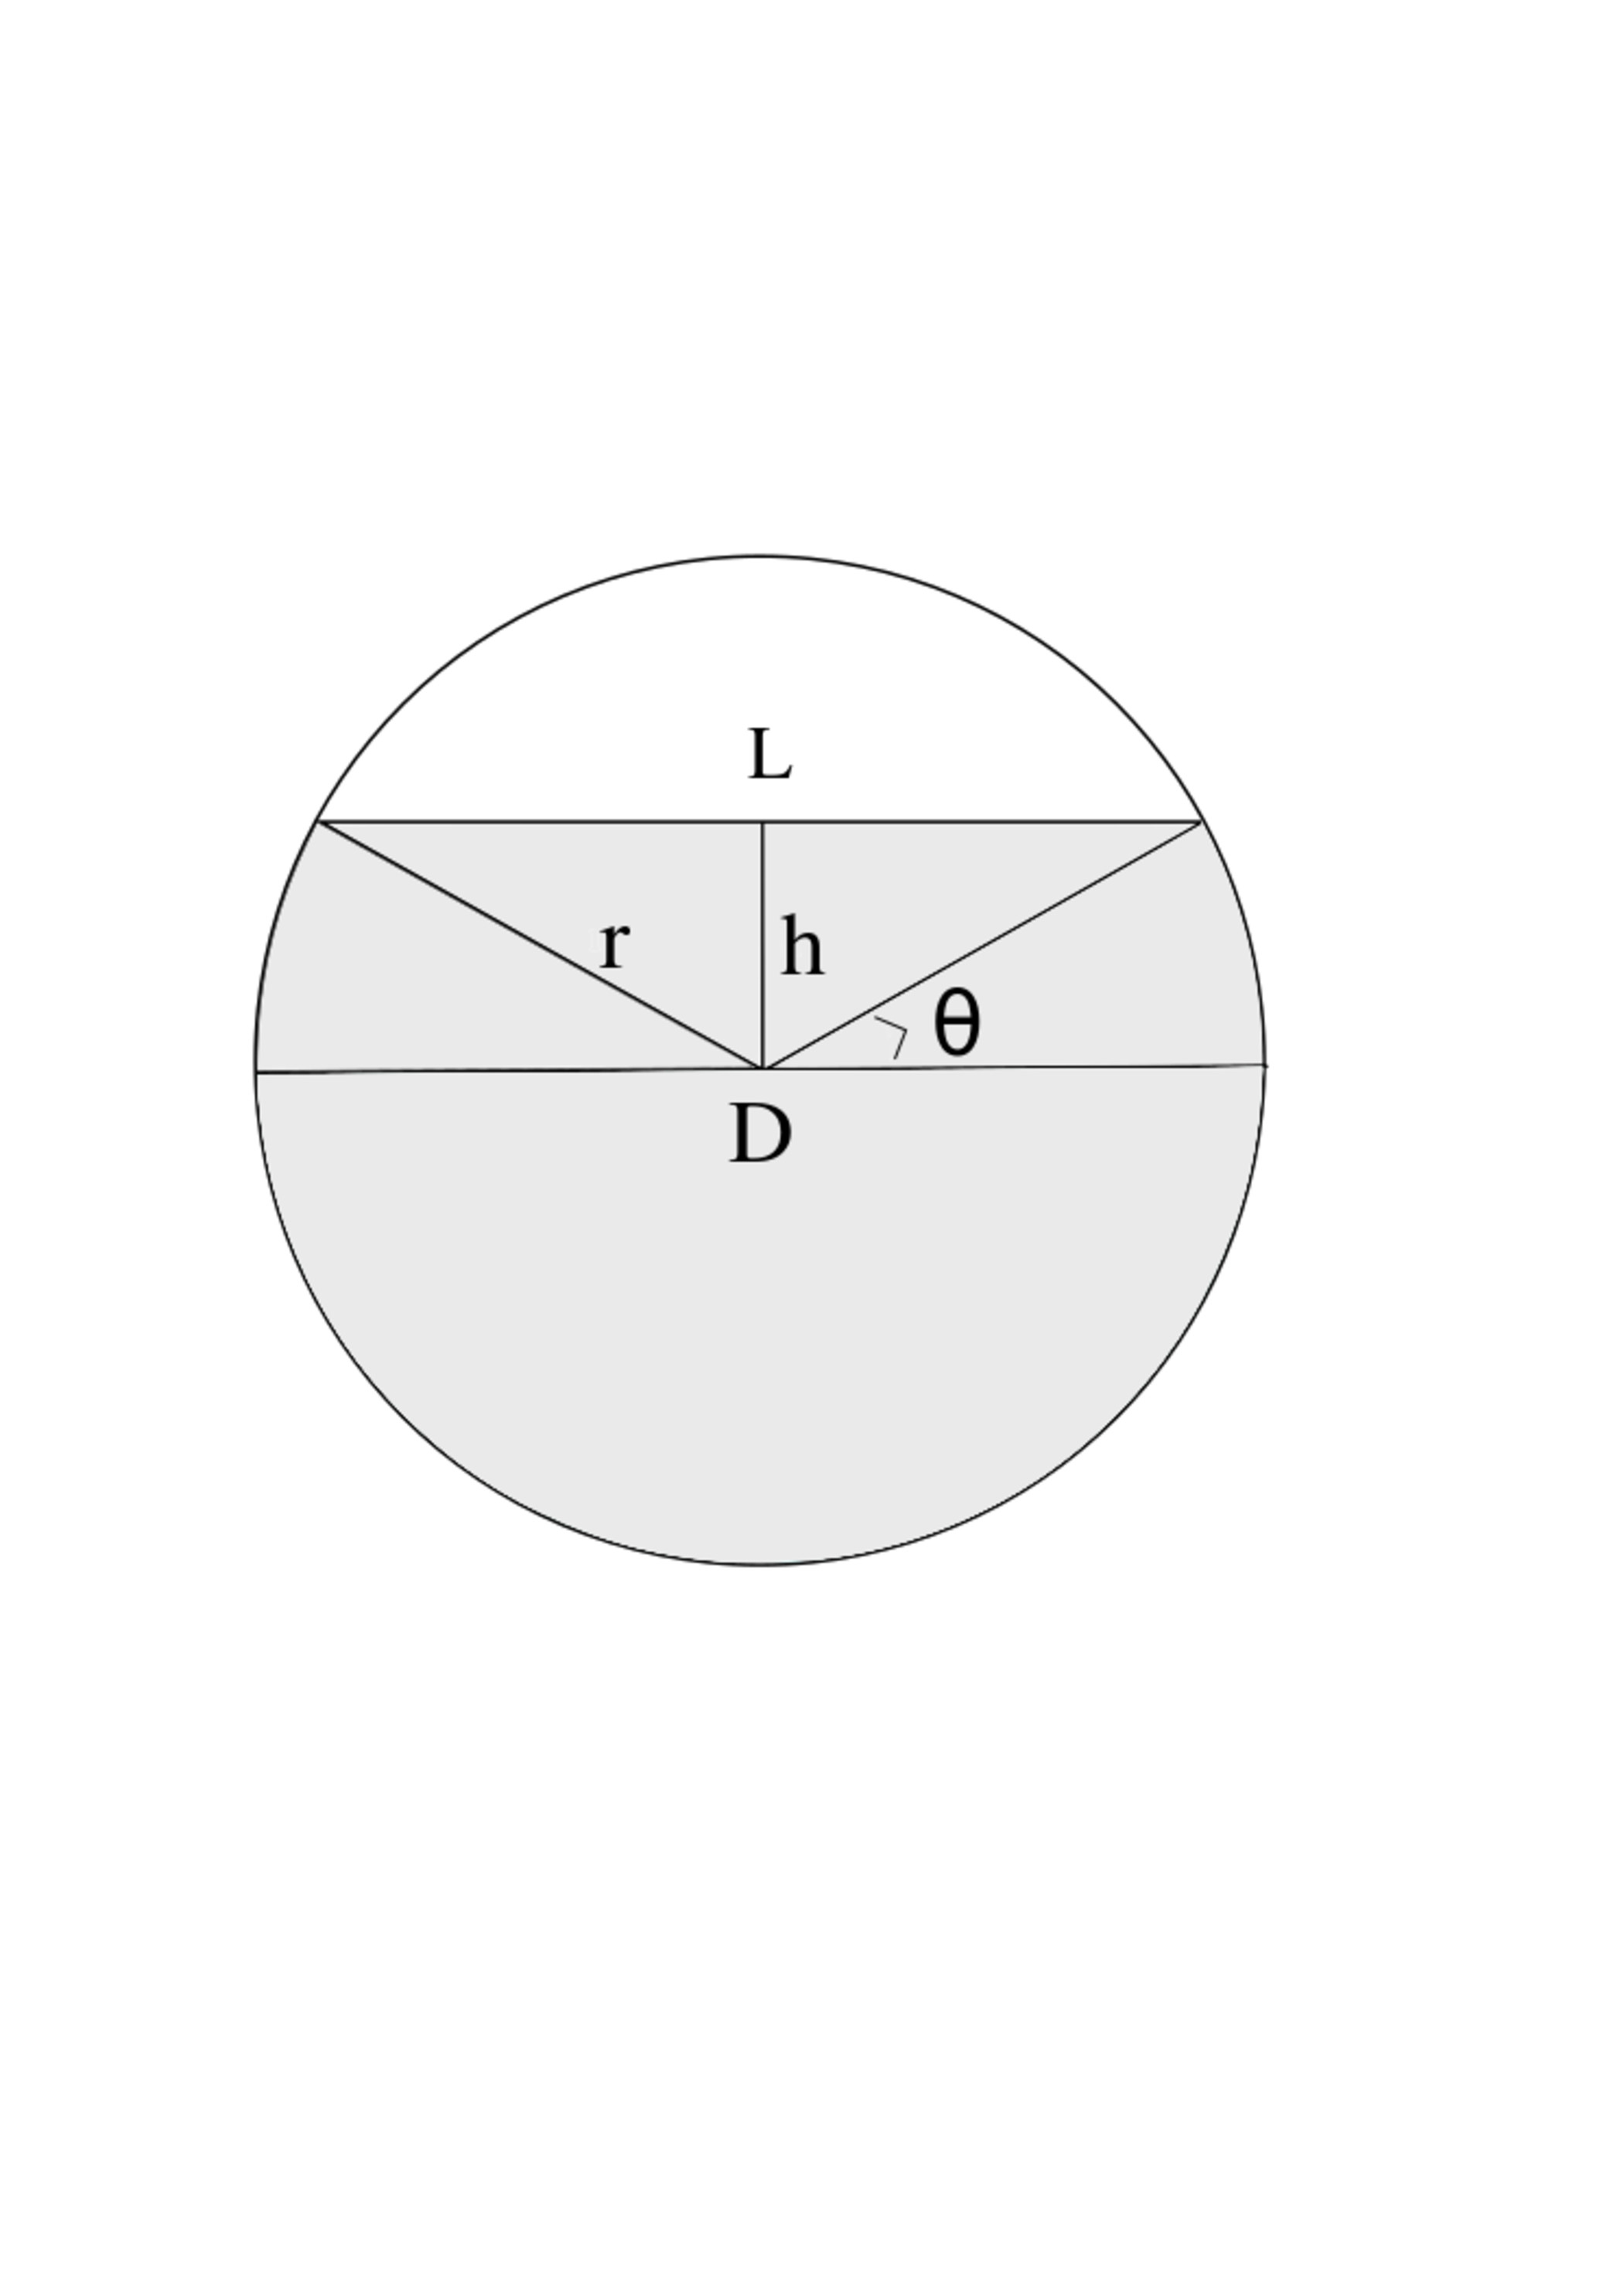
\includegraphics[width=\textwidth]{fig/polishing/fiberdiagram.jpg}
    \caption{Symbols used in the calculation of a fiber cross section, where the shaded area represents the remaining fiber area. Both L and D are subject to measurement errors.}
    \label{fig:fiber}
\end{figure}
\subsubsection{errors in the calculation}
The geometrical error



